\documentclass{article}[11pt]
\linespread{1.5}
\usepackage{fullpage}
\usepackage{amsmath,theorem,amssymb,graphicx, pgfplots, tabularx, placeins}
\usepackage[semicolon,authoryear]{natbib}
\usepackage{caption}
\usepackage{subcaption}
\usepackage{csquotes}



\newcommand{\lb}{\label}
\newtheorem{thm}{Theorem}
\newtheorem{prop}{Proposition}
\newtheorem{definition}{Definition}

\title{The New Keynesian Transmission Mechanism: A Heterogenous Agent Perspective\footnote{We are grateful for helpful comments by Adrien Auclert, L\'idia  Brun, Martin Eichenbaum, Jordi Gal\'i, John Hassler, Jean-Baptiste Michau, Matthew Rognlie, Johan S\"{o}derberg, Karl Walentin, Iv\`{a}n Werning, Andreas Westermark and seminar participants at the IIES, MIT Macro Lunch, Universitat Pompeu Fabra, Sveriges Riksbank, ENTER Jamboree in Mannheim 2015, UiO-NHH Macro Workshop at Norges Bank, SED Annual Meeting 2015 and EEA Annual Meeting 2015. All errors are our own.}}

\author{
  Tobias Broer\footnote{IIES, CEPR. tobias.broer@iies.su.se}\\
  \and
  Niels-Jakob Harbo Hansen\footnote{IIES. nielsjakobharbo.hansen@iies.su.se}\\
  \and
  Per Krusell\footnote{IIES, CEPR, NBER. per.krusell@iies.su.se}\\
  \and
  Erik \"{O}berg\footnote{IIES. erik.oberg@iies.su.se}\\
}
\date{\parbox{\linewidth}{\centering%
  April 29, 2015\endgraf\bigskip
  {\Large \textbf{Preliminary and incomplete - please do not quote!}}\endgraf}}

\begin{document}

\maketitle 



\begin{abstract}
We investigate to what extent household heterogeneity affects the transmission mechanism of monetary policy in the textbook version of the New Keynesian model. For this purpose, we extend the textbook model to contain two classes of households: workers who earn wages, and capitalists who earn profits. We show that the source of nominal rigidities matters greatly for the monetary transmission mechanism in this framework. In the model with only price rigidities, there is no effect on output from monetary policy. This result sharply contrasts with the corresponding representative agent model, in which the large steady state size and countercyclical response of profits explain the procyclical response of labor supply and output. In the model with frictional labor markets, the response of employment and output becomes essentially demand-determined, and the worker-capitalist model behaves closely to the representative agent model. 
\end{abstract}
\newpage
\section{Introduction}
\lb{introduction}
The 3-equation New-Keynesian textbook model is a standard tool for investigating business cycle movements and policies. While having the virtue of being minimal in assumptions, it can still qualitatively match the aggregate responses to various shocks documented in the data. Most notably, it can generate a negative response of output to positive shocks in the nominal interest rate.

We reexamine the transmission mechanism of this model. The standard intuition is that subject to a surprise increase in the nominal interest rate, the real interest rate increase due to sticky prices, and aggregate demand falls due to intertemporal substitution. Since, in the absence of capital, consumption equals output in equilibrium, output falls. However, as in any general equilibrium model, the movement in output must not only be consistent with consumption demand, but also with the supply of factor inputs, which in the 3-equation model solely consist of labor. The supply part of the model is not often discussed but will be the subject of investigation in this paper.

We find that for the response of labor supply, the size and response of firm profits play an essential role. Because prices are sticky, average price markups and profits respond countercyclically to monetary policy shocks. The countercyclical response of profits means that the representative agent experiences a countercyclical income effect, which directly causes a procyclical labor supply response. In addition, under a standard parameterization monopolistic profits make 45 \% of total output in steady state. When returned to a representative agent, this large non-labor income reduces the relative income effect of wages, which reduces the slope of the labor supply schedule.    

We illustrate this mechanism by means of simple modification of the textbook-model to allow for heterogeneity in the functional distribution of income. The modified model has two classes of agents: workers that only receive labor income and capitalists who own the firms. To make the exposition as clear as possible we first consider the case without financial trade between the two agents. In this model, under the standard assumption of King-Plosser-Rebelo (KPR) preferences, labor supply and output is unresponsive to monetary policy shocks. As a robustness exercise, we then allow for financial trade under the assumption of quadratic bond holing costs (to maintain stationarity). Even with small bond holdings costs, the output response is still close to non-existent.

Why does the worker-capitalist model not feature any response of output? Because workers are not given any profits, they do not experience the countercyclical income effect. In addition, because workers consume only labor income, KPR-preferences imply that the income and substitution effect of changes in the wage level cancel, and so labor supply is unresponsive to changes in the real wage. 

The implausible transmission mechanism through profits to employment and output follows from the assumption of frictionless labor markets. We argue that a model with nominal wage rigidities can serve as a better benchmark. In such environments, workers are off their long-run labor supply schedule and supply whatever is demanded at the going wage. The income and substitution effects therefore matter less. We show this in the context of the \citet{Erceg2000} model. In this framework, the standard and the modified worker-capitalist model produce very similar aggregate responses to a monetary policy shock. 

Our discussion is centered around monetary policy shocks. In the last section of the paper, we discuss another impulse-response in which the 3-equation model has been considered successful; the employment response to TFP shocks. Subject to a positive TFP shock, the 3-equation model generates a fall in employment, which is consistent with findings in the VAR evidence \citep{Gali1999,Gali2004,Francis2005,Basu2006}. We show that this impulse-response is also an artifact of profits being redistributed to the representative agent. In the worker-capitalist modification, employment does not move. The mechanism behind the fall in employment in the standard model is the large and procyclical response of profits, which forms a direct income effect sizable enough to cause a depression of labor supply even though wages increase. 
 
Our paper relates directly to two strands in the literature. Most directly, since we highlight a problematic property of the 3-equation model, our analysis relates to a number of studies that uses this model for analysis of the business cycle and business cycle policy. To name a few, \citet{Lorenzoni2009} studies the effect of news shocks. \citet{Christiano2011} analyzes government spending multipliers. \citet{Werning2012} characterize optimal fiscal and monetary policy at the zero lower bound. 

Secondly, our analysis connects the recent literature that has analyzed the effect of household income and wealth heterogeneity in New-Keynesian environments, since our worker-capitalist model can be seen as highly stylized model of the same type of heterogeneity. \citet{Auclert2015} studies amplification of monetary policy through redistribution and heterogeneity in marginal propensities to consume. \citet{McKay2015} studies how the precautionary savings motive affects the responsiveness to forward-guiding monetary policy. \citet{McKay2013} and \citet{Ravn2012a} studies richer model to uncover the effect of job uncertainty and automatic stabilizers. 
\newpage
\section{Two models}
\label{sec:model}
We refer to the model described in \citet{Gali1999} Ch. 3 as the \emph{standard model}. As a tool for investigating the transmission mechanism in the standard model, we will compare the impulse-responses of this model to a model where we give the profit income to a non-working household. We name the latter model the \emph{worker-capitalist model}. In this section we describe the setup of these two models. Apart from the household sector, the models are identical in the way firm set prices and how the central bank sets the interest rate. Since these components are well-known, we will describe them only briefly.  

As for notation, if not otherwise stated we will for any variable $X_t$ denote its steady state value with $\bar X$, its value in the equilibrium under flexible price setting with $X^n$ (the natural equilibrium), its log value with $x_t$, its log deviation from steady state with $\hat x_t$ and its deviation from the flex price equilibrium with $\tilde x_t$.

\subsection{The standard model: The representative household}
The standard model has a representative household. This household derives utility from consuming a final good and disutility from working. It collects wage and profit income and can trade in a risk free nominal bond in zero net supply. The representative household's problem is
\begin{eqnarray}
\max_{C_{t}, B_{t+1}, N_t} && E_0 \sum_{t=0}^{\infty} \beta^t \left( \frac{C_{t}^{1-\sigma}}{1-\sigma}-\frac{N_t^{1+\varphi}}{1+\varphi}\right) \nonumber\\
\lb{rephouse_bc}
\text{s.t.} && P_t C_{t} + Q_{t} B_{t} \leq B_{t-1} + W_t N_t + P_t D_t \nonumber
\end{eqnarray}
where $P_t$ denotes the price level, $C_t$ real consumption, $Q_t$ the nominal price of the bond $B_t$, $W_t$ the nominal wage level, $N_t$ labor supply and $D_t$ real profit income. The solution is characterized by an Euler equation and an intratemporal optimality condition:
\begin{eqnarray}
\lb{std_euler}
Q_{t} &=& \beta E_t \left\{\frac{C^{-\sigma }_{t+1}}{C^{-\sigma }_{t}} \frac{P_t}{P_{t+1}}\right\} \nonumber \\
\lb{std_labor}
\frac{W_t}{P_t}C_{t}^{-\sigma} &=& N_t^{\varphi} \nonumber
\end{eqnarray}
Log-linearizing around the flex-price equilibrium, we find  
\begin{eqnarray}
\lb{std_euler_log}
\tilde c_{t} &=& -\frac{1}{\sigma}(i_t-E_t \pi_{t+1}-\rho) + E_t \tilde c_{t+1} \\
\lb{std_labor_log}
\tilde \omega_t &=& \varphi \tilde n_t + \sigma \tilde c_t
\end{eqnarray}
where $\omega_t=w_t-p_t$, $\rho=-\log \beta$, $i_t=-\log{Q_t}$ and $\pi_t = p_t-p_{t-1}$. 

The goods market clears when
\begin{eqnarray}
C_t = Y_t \nonumber
\end{eqnarray}
where $Y_t$ is total output. The bond market clears when $B_t=0$, which implies that
\begin{eqnarray}
C_t = \frac{W_t}{P_t}N_t+D_t \nonumber
\end{eqnarray}
Log-linearizing around the flex-price equilibrium, we find 
\begin{eqnarray}
\lb{std_mcgoods_log}
\tilde c_t &=& \tilde y_t \\
\lb{std_mcbonds_log}
\tilde c_t &=& \bar S (\tilde \omega_t+\tilde n_t) + (1-\bar S)\tilde d_t
\end{eqnarray}
where $\bar S=\frac{\bar W \bar N}{\bar Y \bar P}$ is the steady state labor income share of output.


\subsection{The worker-capitalist model: The households}
The worker-capitalist model is constructed with the purpose of isolating the effect of profits in the standard model. It has a representative worker and a representative capitalist. The worker can trade in a risk-less bond while the capitalist is constrained to be hand-to-mouth. This simplifying assumption implies that in equilibrium, each household consumes neither more nor less than its factor income, and enables us to ignore the evolution of the wealth distribution. An alternative specification would constrain the worker to be hand-to-mouth while allowing the capitalist to trade in the bond market. These two models have the same implications for the determination of labor supply, since both imply that the worker only consumes labor income in equilibrium. However, as discovered by  \citet{Bilbiie2008}, the model with a constrained worker has no determinate log-linear equilibrium under a standard Taylor rule. To be able to keep the rest of the model exactly the same as the standard model, we therefore constrain the capitalists instead.  

Disallowing financial trade between the two households may seem as a non-innocent assumption. As a robustness check, we will in Section \ref{sec:bond_trade} consider a model where financial trade between the households is allowed. For reasonable calibrations, the results are not significantly affected.

The worker derives utility from consuming the final good and disutility from working. She collects wage income and can trade a in a risk free nominal bond. In contrast to the representative household in the standard model, she does not receive any profit income. The worker's problem is
\begin{eqnarray}
\max_{C_{wt}, B_{wt+1}, N_t} && E_0 \sum_{t=0}^{\infty} \beta^t \left( \frac{C_{wt}^{1-\sigma}}{1-\sigma}-\frac{N_t^{1+\varphi}}{1+\varphi}\right) \nonumber \\
\lb{worker_bc}
\text{s.t.} && P_t C_{wt} + Q_{t} B_{wt} \leq B_{wt-1} + W_t N_t \nonumber
\end{eqnarray} 
The solution is characterized by an Euler equation and an intratemporal optimality condition:
\begin{eqnarray}
\lb{wc_euler}
Q_{t} &=& \beta E_t \left\{\frac{C^{-\sigma }_{wt+1}}{C^{-\sigma }_{wt}} \nonumber \frac{P_t}{P_{t+1}}\right\} \\
\lb{wc_labor}
\frac{W_t}{P_t}C_{wt}^{-\sigma} &=& N_t^{\varphi} \nonumber
\end{eqnarray}
Log-linearizing around the flex-price equilibrium, we find 
\begin{eqnarray}
\lb{wc_euler_log}
\tilde c_{wt} &=& -\frac{1}{\sigma}(i_t-E_t \pi_{t+1}-\rho) + E_t \tilde c_{wt+1} \\
\lb{wc_labor_log}
\tilde{\omega}_t &=& \varphi \tilde n_t + \sigma \tilde c_{wt}
\end{eqnarray}
The capitalist receives profits and consumes them hand-to-mouth. The capitalist's problem is  
\begin{eqnarray}
\max_{C_{ct}} && E_0 \sum_{t=0}^{\infty} \beta^t \left( \frac{C_{ct}^{1-\sigma}}{1-\sigma}\right) \nonumber \\
\lb{worker_bc}
\text{s.t.} && P_t C_{wt} \leq P_t D_t \nonumber
\end{eqnarray}
The goods market clears when
\begin{eqnarray}
C_{wt}+C_{ct} \leq Y_t \nonumber
\end{eqnarray}
where $Y_t$ is total output.  The bond market clears when $B_{wt} = 0$ which implies that 
\begin{eqnarray}
C_{wt} &\leq& \frac{W_t}{P_t}N_t \nonumber
\end{eqnarray}
Log-linearizing around the flex-price equilibrium, we find 
\begin{eqnarray}
\lb{wc_mcgoods_log}
\bar S \tilde c_{wt}+ (1-\bar S) \tilde c_{ct} &=& \tilde y_t \\
\lb{wc_mcbonds_log}
\tilde c_{wt} &=& \tilde \omega_t + \tilde n_t
\end{eqnarray}
where $\bar S=\frac{\bar W \bar N}{\bar Y \bar P}$ is the steady state labor income share of output.

\subsection{Other model components}
The production sector, the firm pricing problem and the central bank response function is identical in the two models and follows \citet{Gali1999} Ch. 3. We describe them briefly here. 

There is a representative firm that produces the final good $Y_t$ by combining a continuum of intermediate goods $Y_{it}$ through the Dixit-Stiglitz aggregator with elasticity of substitution $\epsilon_p$. These intermediate goods are produced by a continuum of firms, indexed by $i$, with technology $Y_{it}=A_t N_{it}^{1-\alpha}$. The intermediate goods producers set their prices to maximize present discounted profits with the market discount factor $Q_t$. They can, however, only reset their prices with probability $1-\theta_p$ in every period. From these assumptions we can derive a log-linear relationship between inflation and the deviation of average marginal cost from steady state:
\begin{eqnarray}
\pi_t = \beta E_t \pi_{t+1}+\lambda \hat{mc}_t
\end{eqnarray}  
where $\lambda = \frac{(1-\theta_p)(1-\beta \theta_p)}{\theta_p} \frac{1-\alpha}{1-\alpha+\alpha \epsilon_p}$. 

The model is closed by assuming that a central bank sets the interest rate according to a log-linear Taylor rule:
\begin{eqnarray}
i_t = \rho + \phi_{\pi}\pi_t + \phi_{y}\tilde y_t +\nu_t
\end{eqnarray}

\subsection{Parameterization}
All parameters are the same in the two models. We choose the same calibration as that in \citet{Gali2009} Ch. 3. A time period should be interpreted as a quarter of a year. We set an elasticity of intertemporal substitution $1/\sigma=1$ (which is a special case of KPR preferences), Frisch elasticity $\varphi=1$, $\alpha=1/3$, $\epsilon_p=6$, $\theta_p=2/3$, $\beta=0.99$. For the Taylor rule, we set $\phi_{\pi}=1.5,\phi_{y}=0.125$. 

For this parameterization, it is easily confirmed that the log-linear equilibrium system of both models has a unique stable solution. 


\newpage
\section{Impulse-responses to a monetary policy shock}
\label{sec:results}
We now consider how the two models respond to the same innovation in the policy rate. We assume that innovations in the policy rate follow the process
\begin{eqnarray}
\nu_t &=& \rho_{\nu} \nu_{t-1}+\epsilon_{\nu t} \nonumber
\end{eqnarray}
with $\rho_{\nu}=0.5$. We feed a positive $25$ basis point shock to the models. The responses are plotted in Figure \ref{fig_monetary_std_nt}. In the figure, we plot deviations from the flex price equilibrium. We will refer to the these deviations as ''gaps''.

As can be seen in Figure \ref{fig_monetary_std_nt}, the models respond qualitatively similar in terms of the real interest rate gap, inflation, real wages and profits. However, in the standard model, there is a substantial negative response of output and employment whereas in the worker-capitalist model, there is no response at all.

We start analyzing the responses of the worker-capitalist model, as the insights from this exercise will better enable us to uncover the mechanism in the standard model. Looking at the right-hand side of \ref{fig_monetary_std_nt}, we see that in response to the surprise increase in the nominal interest rate, the real interest rate increases. From the Euler Equation \eqref{wc_euler_log}, we then know that the worker consumption gap must start out negative to follow an upward sloping path. The worker income gap must follow the same path, as worker consumption equals worker income in equilibrium. Hence, either wages, labor supply or both must initially fall. We see that it is only real wages that falls while labor supply does not move. 

Why is there no response in labor supply? Because of the parametric assumption of $\sigma=1$ (KPR-preferences), the income and substitution effect with respect to changes in the wage level cancel. To see this, insert the market clearing condition \eqref{wc_mcbonds_log} in the intratemporal optimality condition \eqref{wc_labor_log}:
\begin{eqnarray}
&& \varphi  \tilde n_t + \sigma  \tilde c_t =  \tilde \omega_t \nonumber \\
\Rightarrow  && \tilde \varphi n_t + \sigma ( \tilde \omega_t+ \tilde n_t) =  \tilde \omega_t \nonumber \\
\Leftrightarrow && (\varphi+\sigma)  \tilde n_t = (1-\sigma) \tilde \omega_t \nonumber
\end{eqnarray} 
and under $\sigma=1$:
\begin{eqnarray}
\tilde n_t = 0 \nonumber
\end{eqnarray}
Since labor supply cannot move, the fall in worker consumption matches the fall in wages. And because wages fall, so does the marginal cost of production, which leads to a fall in inflation and an increase in profits. The countercyclical response of profits, however, has no effect on the equilibrium since it is consumed by the hand-to-mouth capitalists.

Having explained the responses in the worker-capitalist model, it is now easy to understand the standard model responses. As in the worker-capitalist model, the real interest rate gap increases, which leads to a fall in the consumption gap. There is also a fall in the real wage gap and an increase in the profit gap. However, in contrast to the worker-capitalist model now hours worked and the output gap decreases. To explain this, we again insert in the market clearing condition \eqref{std_mcbonds_log} in the intratemporal optimality condition \eqref{std_labor_log}:
\begin{eqnarray}
&& \varphi \tilde n_t + \sigma \tilde  c_t =  \tilde \omega_t \nonumber\\
\Rightarrow  &&\varphi \tilde  n_t + \sigma \left( \bar S( \tilde \omega_t+ \tilde n_t) + (1-\bar S)\tilde d_t   \right) =  \tilde \omega_t \nonumber \\
\Leftrightarrow && (\varphi+\sigma \bar S)  \tilde n_t = (1-\sigma \bar S) \tilde \omega_t -\sigma (1-\bar S) \tilde d_t \nonumber
\end{eqnarray}
and under $\sigma=1$:  
\begin{eqnarray}
\lb{std_response}
\tilde n_t = \frac{1-\bar S}{\varphi+\bar S}(\tilde \omega_t-\tilde d_t) \nonumber
\end{eqnarray}  
where $\frac{1-\bar S}{\varphi+\bar S}$ is decreasing in $\bar S$ on the unit interval. Under the current parameterization, the labor share of income is close to $55$ per cent. Because profits increase in response to the shock, the representative household experiences a direct income effect which depresses labor supply. This effect is naturally decreasing in the steady state labor share, as seen in \eqref{std_response}. We also see that as the labor share decreases, the response of labor supply to changes in the real wage increases. With a larger profit income share in steady state, the relative income effect of wage changes is depressed. The labor supply schedule then become less downward sloping, and labor supply becomes more responsive to changes in the real wage level, even though we have KRP preferences.  

The standard model is thus capable to generate negative responses of employment and output to a positive innovation in the policy rate because the steady share of profit is substantial and because these profits respond countercyclically. When returned to the representative household, its responsiveness of labor supply to real wages increase while it experiences a negative income effect to monetary policy shocks. 

This transmission mechanism does not seem reasonable. Few households have substantial non-labor income and there is, to our knowledge, no evidence that profit income responds procyclically to monetary policy shocks.\footnote{The VAR evidence presented by \citet{Christiano2005} shows that firm profits respond procyclically to monetary policy shocks.} 






\newpage
\section{Robustness: Allowing financial trade}
\label{sec:bond_trade}
In the setup of the worker-capitalist model, we disallowed financial trade between the two households. We made this assumption to simplify the analysis. As a robustness exercise, we will in this section consider the case where we allow financial trade. 

Without further assumptions, allowing the capitalist to trade in the bond market implies that the model becomes non-stationary. In response to a monetary policy shock, we have seen that real wages respond procyclically and profits respond countercyclically. One household will therefore become indebted to the other. The consumption smoothing motive makes this indebtedness permanent. Hence, after a monetary policy shock, the equilibrium does not converge back to the steady state from which it started.

To allow for financial trade in the model we therefore assume that the capitalist faces quadratic bond holding costs, which ensures that the capitalist holds zero financial wealth in the long-run equilibrium. This assumption is commonly used to close two-country international macro models, see e.g. \citep{Schmitt-Grohe2003}.

Thus, we change the capitalist problem described in Section \ref{sec:model} to 
\begin{eqnarray}
\max_{C_{ct}, B_{ct}} && E_0 \sum_{t=0}^{\infty} \beta^t \left( \frac{C_{ct}^{1-\sigma}}{1-\sigma}\right) \nonumber \\
\lb{worker_bc}
\text{s.t.} && P_t C_{wt} + Q_t B_{ct} \leq B_{ct-1}+P_t D_t-\frac{\zeta}{2}B_{ct-1}^2 \nonumber
\end{eqnarray}
with the associated Euler equation
\begin{eqnarray}
\lb{bt_euler}
Q_{t} &=& \beta E_t \left\{\frac{(1-\zeta B_{ct}) C^{-\sigma }_{ct+1}}{C^{-\sigma }_{ct}} \nonumber \frac{P_t}{P_{t+1}}\right\} \nonumber
\end{eqnarray}
Log-linearizing around the flex-price equilibrium, we find 
\begin{eqnarray}
\lb{bt_euler_log}
\tilde c_{ct} &=& -\frac{1}{\sigma}(i_t-E_t \pi_{t+1}-\rho) + E_t \tilde c_{ct+1} +\zeta Y^n_t \tilde b_{ct}
\end{eqnarray}
where $\tilde b_{ct}$ is defined as $\tilde b_{ct} = \frac{B_{ct}}{Y^{n}_t}$, i.e. the private debt-to-GDP ratio, where GDP is measured by its flex price value.

The goods and bond market clearing conditions are now
\begin{eqnarray}
C_{wt}+C_{ct}+\frac{\zeta}{2}B_{ct-1}^2=Y_t  \nonumber \\
B_{ct}+B_{wt}=0 \nonumber 
\end{eqnarray}
In the flex-price equilibrium, the labor share of GDP is constant and so there are no gains from financial trade. Thus $B^n_{ct}=B^n_{wt}=0$. Using this and log-linearizing around the flex-price equilibrium, we find 
\begin{eqnarray}
\lb{bt_mcgoods_log}
\bar S \tilde c_{wt}+ (1-\bar S) \tilde c_{ct} &=& \tilde y_t  \\
\lb{bt_mcbonds_log}
\tilde c_{wt} &=& \tilde \omega_t + \tilde n_t
\end{eqnarray}
The rest of the worker-capitalist model is unaffected.\footnote{Discuss convergence? With $\zeta \rightarrow 0$ the log-linear solution to of this model converges to that of the standard model. With $\zeta \rightarrow \infty$ it converges to that of the worker-capitalist model without trade.}

Before showing results, we need to calibrate $\zeta$. Because wages respond strongly and procyclically and profits respond strongly and countercyclically, the gains from trade between the capitalist and the worker after a monetary shock are very large. When $\zeta \rightarrow 0$, the debt-to-GDP ratio increases from 0 to a peak response of $92$ percent, or a debt-to-worker income of $166$ percent, to a 25 basis point shock with half-life of one quarter. We calibrate $\zeta$ by constraining the response in this variable. Although still implausibly large, we constrain the debt-to-GDP to not respond more than $10$ percent at peak, which implies that $\zeta=3$. 

We feed in the same monetary shock as in the previous section. The responses are plotted in Figure \ref{fig_monetary_std_bt}. As can be seen, the worker-capitalist model still has virtually no response in output and employment. Why is this? Because the debt response is limited to 10 percent of GDP, worker consumption is still close to labor income in every period. Hence, the determination of labor supply is similar to the model without financial trade between the two households. Workers do not experience the positive income effect coming from the increase in profits. And with KRP-preferences, the income and substitution effect is still approximately of the same size, and there is no response to changes in the wage level. 


\newpage
\section{Rigid wages: A solution}
\label{sec:wage_rigidity}

%We have discussed the transmission mechanism of monetary policy shocks in the standard model. By contrasting this model to a simple heterogeneous agent model that separates workers from capitalist, we have shown the distribution and response of profits is instrumental for the output response. 

The only sources of frictions in the standard model are the assumptions of rigid price setting and monopolistic competition. Labor markets are assumed to operate without any frictions. This assumption is key for the transmission mechanism. With households reoptimzing their labor supply decision at high frequency, profits serve the dual role of producing a countercyclical income effect, as well as driving a wedge between labor income and consumption in the steady state. If constraining the households to not be able to reoptimize at high frequency, as is the case with sufficiently rigid wage setting, we should not expect this transmission mechanism to be operating.

In this section, we therefore explore whether assuming rigid wage setting escapes the implausible transmission mechanism of the standard model. We focus on one particular way of introducing rigid wage setting, the assumption of constant resetting probabilities (the ''Calvo model'') introduced by \citet{Erceg2000}, which is frequently used in the literature. We will explore the role of profits in the same fashion as before; by comparing the impulse-responses of the representative agent economy to the worker-capitalist economy (without financial trade).

Constant wage resetting probabilities take the same form in both models. We only discuss the setup briefly here, for a full specification see \citet{Gali1999} Ch. 6. In the standard (worker-capitalist) model, we assume that there is a continuum of ex ante identical households (workers), indexed by $j$, that can trade complete state-contingent consumption claims among themselves. Each household (worker) is assumed to be a monopolistic supplier of its particular labor type and chooses $W_{jt}$. There is a representative intermediate aggregate factor producer that combines the particular labor types $N_{jt}$ with the Dixit-Stiglitz aggregator into an aggregate factor input $N_t$, with elasticity of substitution $\epsilon_w$. As a consequence, each household (worker) faces labor demand schedule of the form
\begin{eqnarray}
\lb{labor_demand}
N_{jt}=\left(\frac{W_{jt}}{W_t}\right)^{-\epsilon_w} N_t
\end{eqnarray}
Under frictionless wage setting, households (workers) each period optimize over $W_t$ to maximize their present discounted lifetime utility. However, households (workers) can only reset their wages with probability $1-\theta_w$ in each period. Conditional on resetting, households (workers) choose a wage level that maximizes their present discounted lifetime utility. Conditional on not being able to reset, they are constrained to supply the labor demanded given by \eqref{labor_demand}.

From these assumptions, in addition to the model equations described in Section \ref{sec:model}, the equilibria of both models are characterized by a ''wage Phillips curve'' and an accounting equation for the evolution of real wages:
\begin{eqnarray}
\pi^w_t &=& \beta E_t \pi^w_{t+1} + \lambda_w \hat \mu_{t} \\
\omega^w_t &=& \omega_{t-1} + \pi^w_{t} - \pi_t + \Delta \omega^n_t
\end{eqnarray}
where $\lambda_w=\frac{(1-\theta_w)(1-\beta \theta_w)}{\theta_w} \frac{1}{1+\epsilon_w \varphi}$ and $\hat \mu_{t}$ is the log deviation of real wages from the average marginal rate of substitution between consumption and leisure for the households (workers).

As in \citet{Gali1999}, we set $\epsilon_w=6$ and $\theta_w=\frac{3}{4}$, which correspond to an average wage duration spell of four quarters. We feed in the same monetary shock as in the previous sections. The responses are plotted in Figure \ref{fig_monetary_std_nt_rigidwages}.

Before comparing the responses of the standard and worker-capitalist model, we discuss how adding wage rigidities in the standard model changes the responses compared to the flex price model responses shown on the left hand side of Figure \ref{fig_monetary_std_nt}. Adding wage rigidities to the standard model changes the magnitude of several responses. Most notably, it almost eliminates the response in real wages completely, as well as making the response of profits procyclical. The reason is that with rigid wage setting, nominal wages respond very little to the shock. Hence, nominal marginal costs of the intermediate goods firms respond only little. In response, the inflation response is muted but sufficiently strong to almost close the real wage gap. As the real wage gap is almost zero, the movement of profits is solely determined by the movement in output. Profits decrease because production decreases, but the effect is mitigated due to diminishing returns to scale.       

Turning to the comparison of the responses between the standard and the worker-capitalist model, we see that they are almost indistinguishable. With an average wage resetting duration of 4 quarters, the income and substitution effects matter less for the determination of hours worked at the shorter horizon. The majority of households (workers) are instead constrained to supply whatever labor is demanded from equation \eqref{labor_demand}. Labor demand follows directly from consumption demand, as labor is the sole factor of production. Thus, in response to the decline in consumption demand coming from the positive real interest rate gap in both models, output and hours worked are thus forced to adjust. 

%That profit response matters for the similarity of the model responses. Because of its small response, aggregate consumption demand moves in accordance with labor income in both models. In a counterfactual thought-experiment where profit had showed a large countercyclical response, as in the model withut wage rigidities, the aggregate consumption demand gap would have been small, and so       

Assuming rigid wages thus seem to offer a solution to the implausible transmission mechanism in the textbook 3-equation model. In the appendix, we show that the difference between the standard and the worker-capitalist model is decreasing in  $\theta_w$, which means that strength of this solution is increasing in the degree of wage rigidities. Whether the actual economies feature substantially rigid wage setting at the business cycle frequency is an empirical question to which we do not contribute in this paper. However, in light of our findings, to have accurate measures of the degree of rigidity seems important for proceeding with these class of model.    

    
  
  



  


\newpage
\section{TFP shocks}
\label{sec:tfp}

Our paper has centered around the transmission mechanism of the standard model to monetary policy shocks. However, as we showed in Section \ref{sec:results}, without the redistribution of profits to the representative household, labor supply is unresponsive to any movement in real wages. This is because without any non-labor income, KPR preferences implies that the income and substitution effect cancel with respect to changes in the wage level. 

We follow this insight to investigate the transmission mechanism from TFP shocks to employment. In contrast to standard real business cycle models, the three-equation new-Keynesian model generates a fall in employment in response to a TFP shock. This impulse-response has been documented in US data \citep{Gali1999,Gali2004,Francis2005,Basu2006}, and has been interpreted as evidence in favor of the new-Keynesian model. 

We proceed in the same fashion as in Section \ref{sec:results}. We consider how the standard and the worker-capitalist models respond to the same innovation in TFP. We assume that innovations in TFP follows the process
\begin{eqnarray}
a_t &=& \rho_{a} a_{t-1}+\epsilon_{a t} \nonumber
\end{eqnarray}
with $\rho_{\nu}=0.9$. We feed a positive $1$ percentage point shock to the models. The responses are plotted in Figure \ref{fig_tfp_std_nt}. Note that in the figure, we do not plot deviations from the flex price equilibrium, but rather deviations from steady state.

As seen in Figure \ref{fig_tfp_std_nt}, the standard model generates a fall in hours worked to the positive innovation in TFP. On the demand side, this response is often interpreted as an effect of the (suboptimal) Taylor rule. In response to the rise in TFP, the unit marginal cost of production falls, which generates a fall in inflation. The central bank then stimulates the economy through the Taylor rule, but not sufficiently to close the real interest rate gap. Although output rises, we then see a fall in the output gap and in hours worked. 

Turning to the supply side, the increase in real wages has a positive effect on labor supply, ceteris paribus. This effect arises due to profit income being large in steady state, so that the relative income effect of wages is depressed. The fall in hours must therefore be a consequence of the large increase in profits, which brings a positive income effect. 

Again, this transmission mechanism does not survive the worker-capitalist model. In this model, workers do not experience the positive income effect from the rise in profits. Workers only experience the rise in wages, but with KPR preferences, this does not affect labor supply. Hence, it is not only the design of monetary policy that is crucial for the response in hours in the standard model, but also the income effect from the large rise in profits.

\newpage
\section{Discussion}
\label{sec:discussion}
\newpage
\bibliographystyle{apalike}
\bibliography{../bibtex/bibtex}
\clearpage
\appendix
\section{Figures}
\lb{figures}

\begin{figure}[ht] 
\centering 
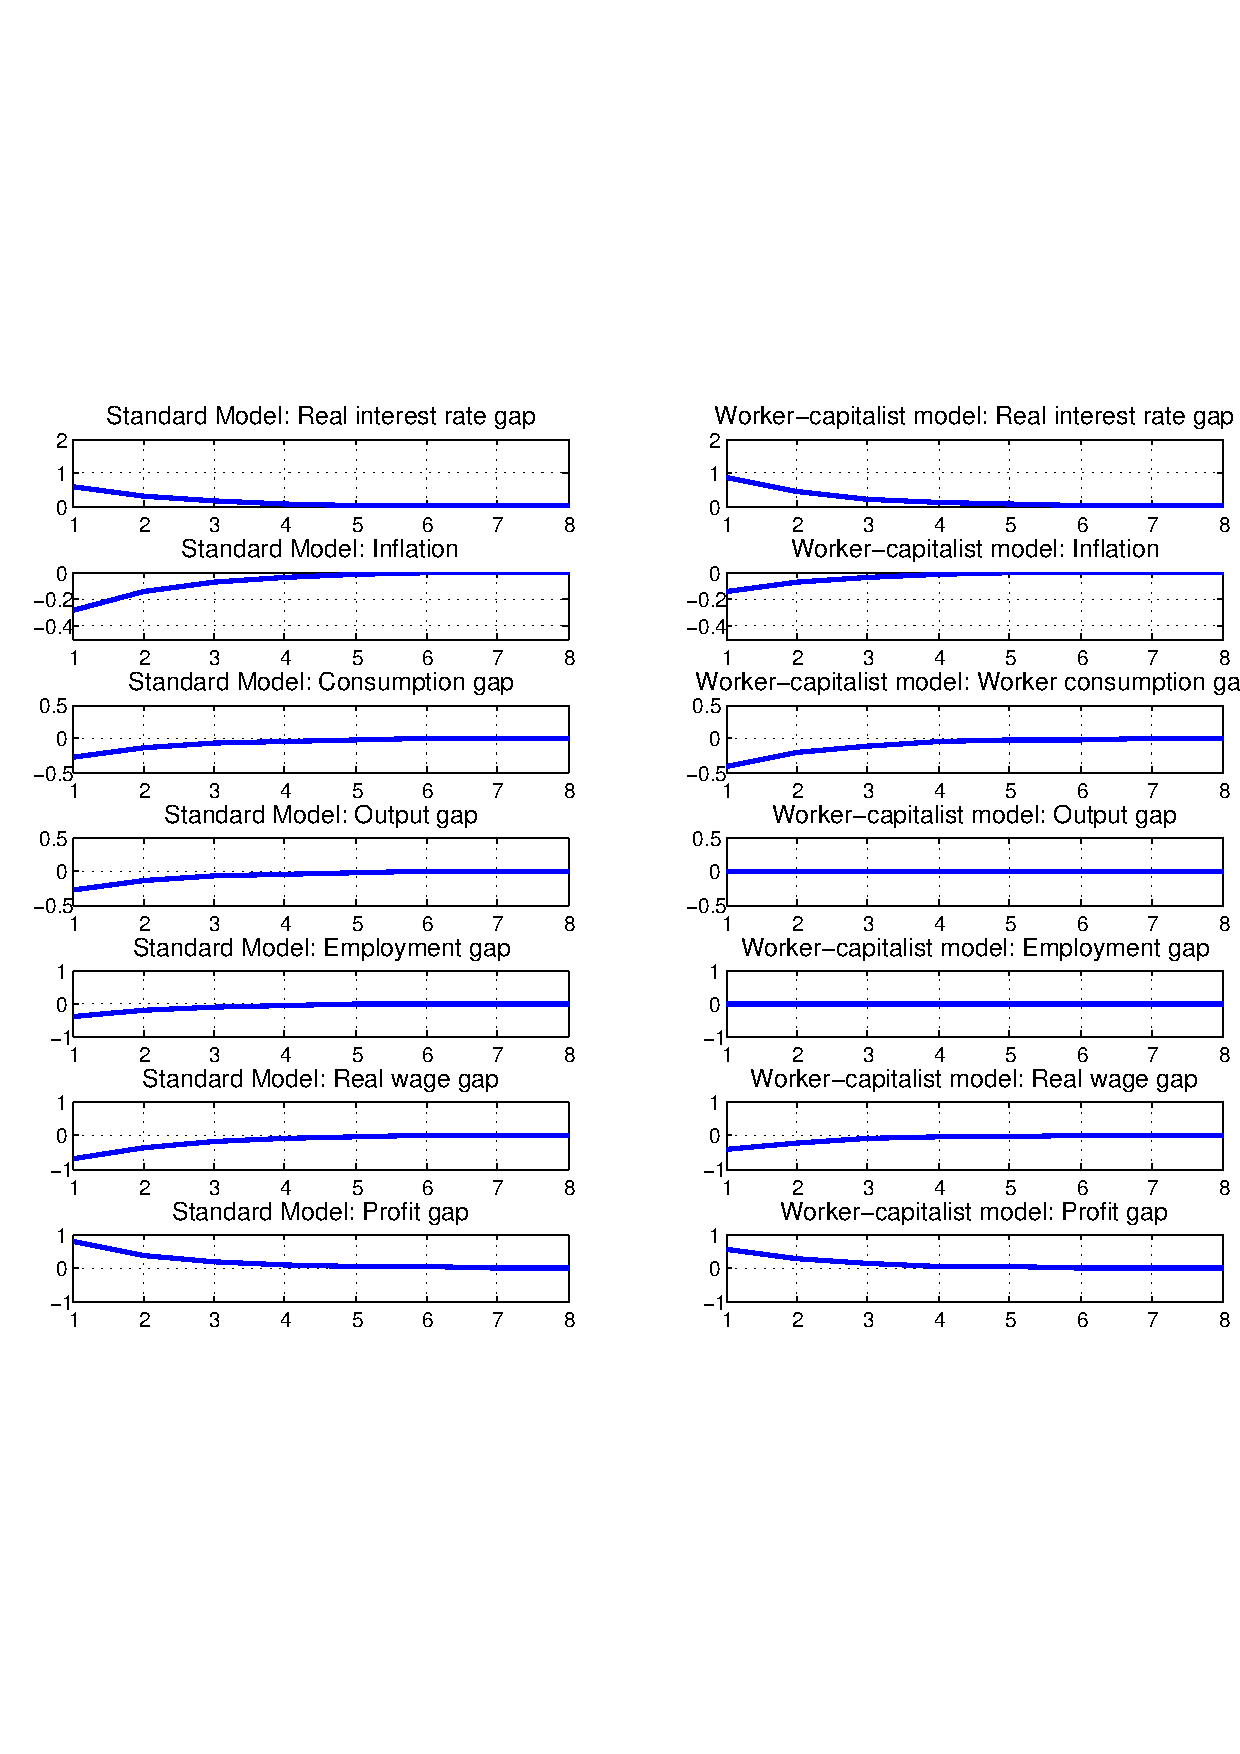
\includegraphics[trim=0cm 7cm 0cm 6cm, clip, width=\textwidth]{./figures/monetary_std_nt.pdf} 
\caption{Equilibrium responses to positive 25 basis shock in the policy rate. The left panel shows the standard model, the right panel the worker-capitalist model. Inflation and interest rates are expressed in yearly terms, while the other variables are expressed in quarterly terms.} 
\label{fig_monetary_std_nt} 
\end{figure}

\begin{figure}[ht] 
\centering 
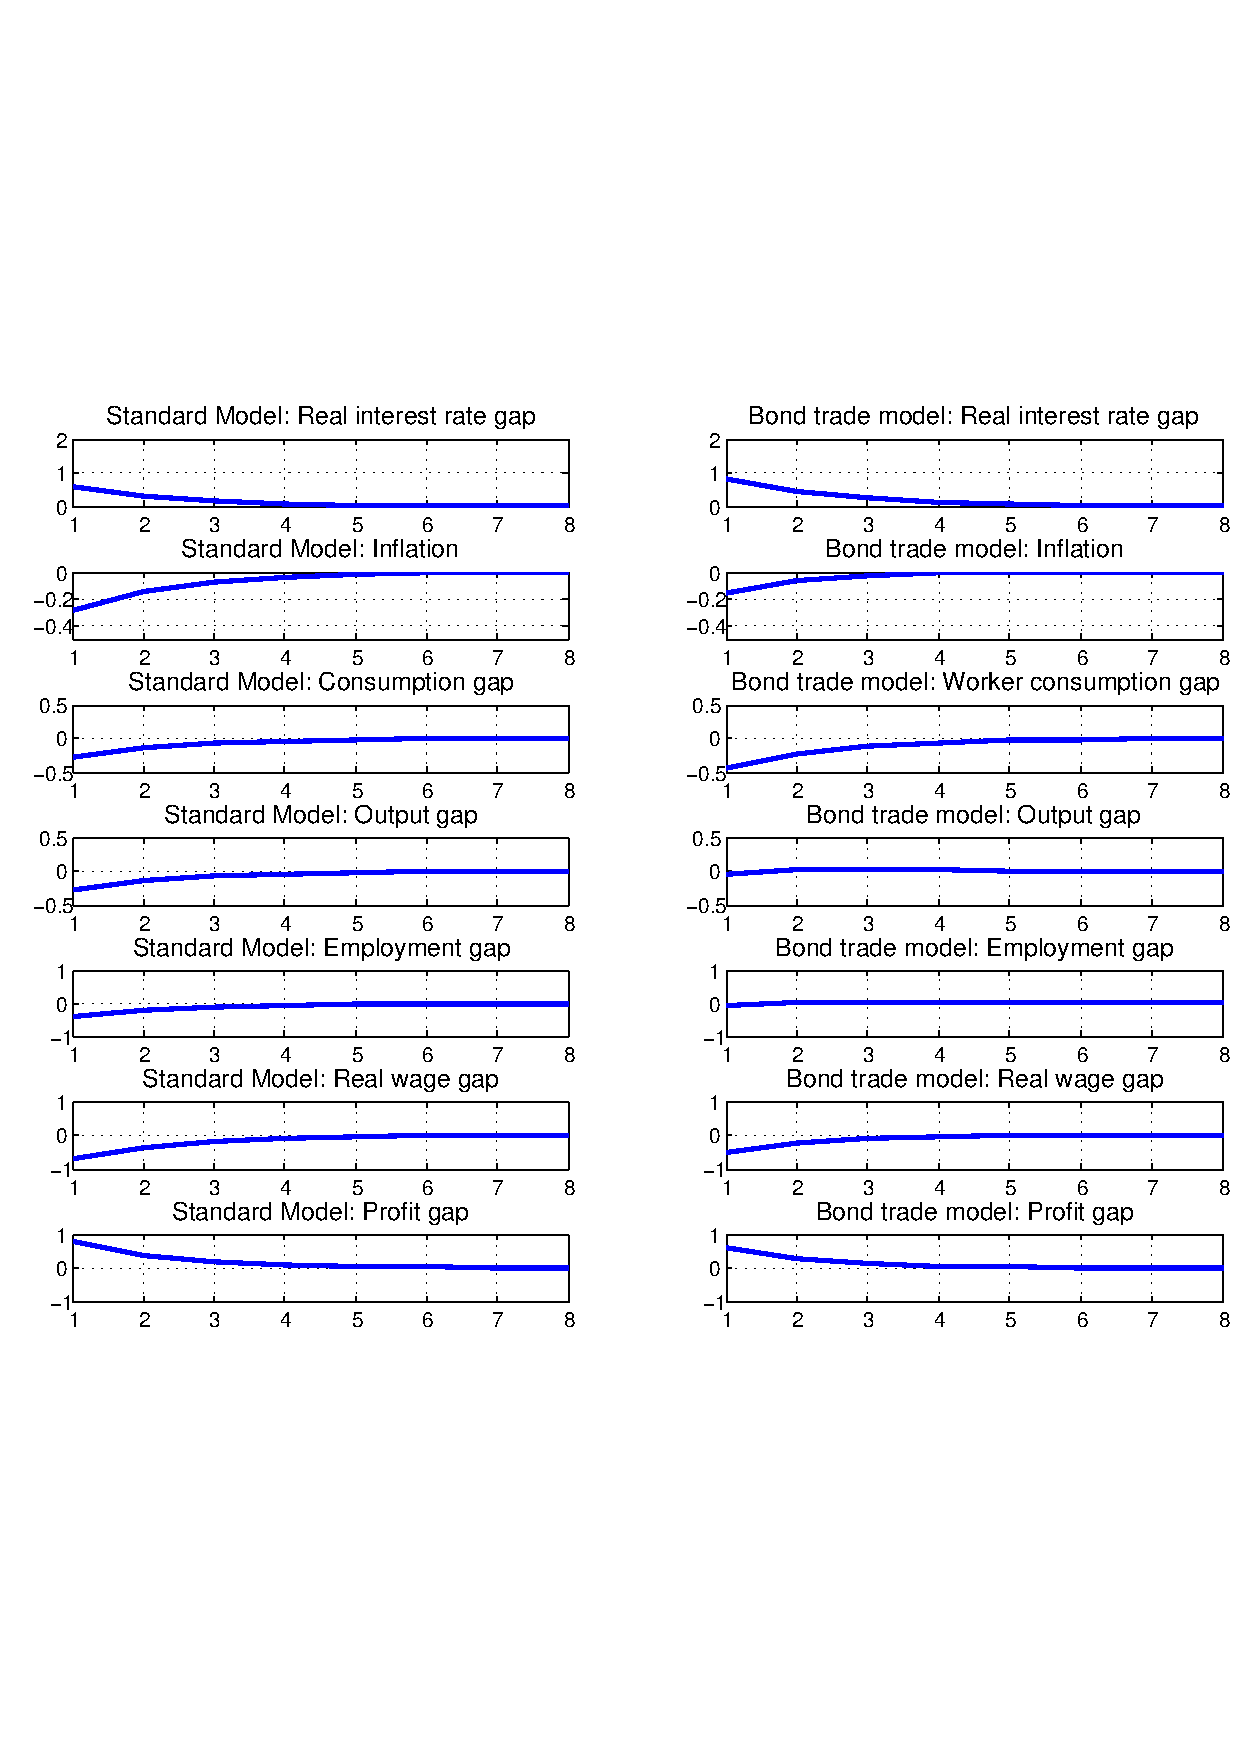
\includegraphics[trim=0.3cm 7cm 0cm 6cm, clip, width=\textwidth]{./figures/monetary_std_bt.pdf} 
\caption{Equilibrium responses to positive 25 basis shock in the policy rate. The left panel shows the standard model, the right panel the worker-capitalist model with financial trade. Inflation and interest rates are expressed in yearly terms, while the other variables are expressed in quarterly terms.} 
\label{fig_monetary_std_bt} 
\end{figure}

\begin{figure}[ht] 
\centering 
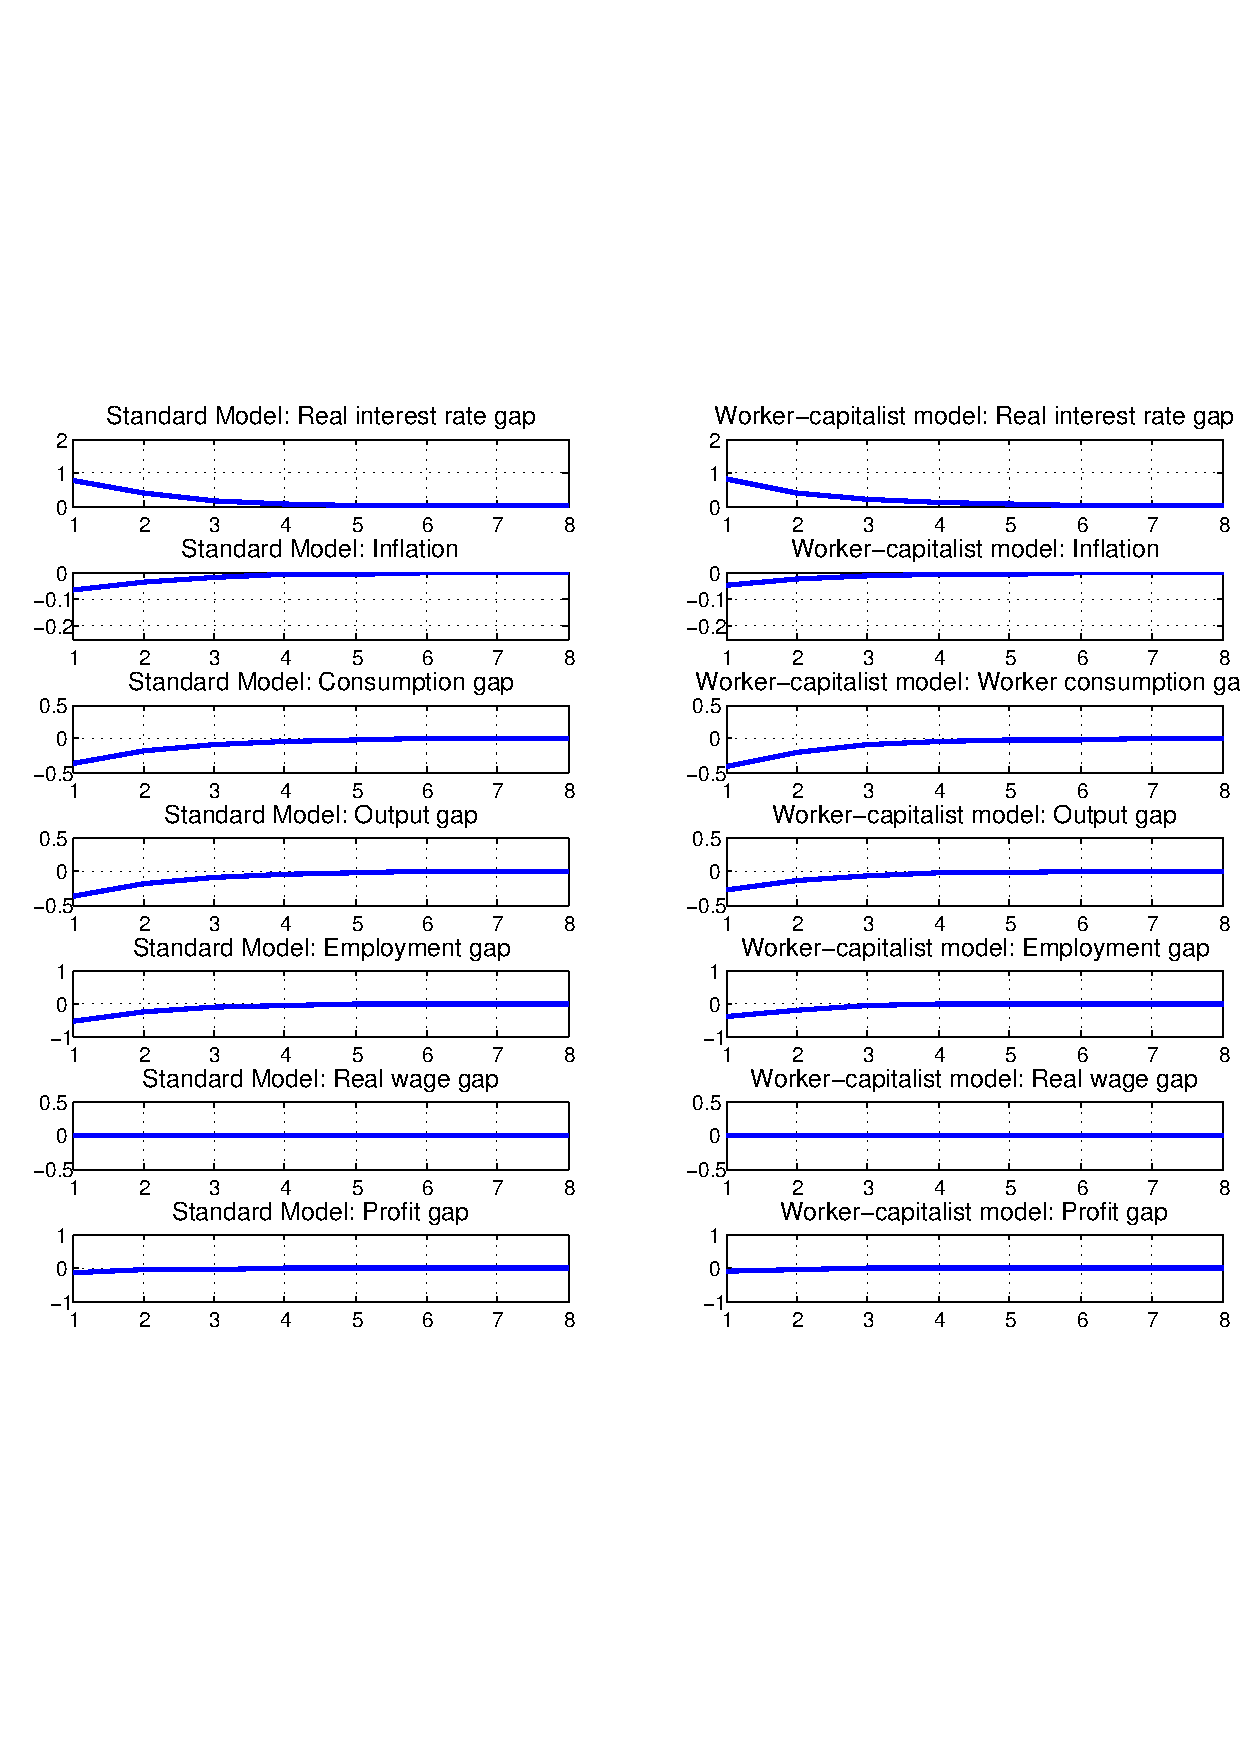
\includegraphics[trim=0.3cm 7cm 0cm 6cm, clip, width=\textwidth]{./figures/monetary_std_nt_rigidwages.pdf} 
\caption{Equilibrium responses to positive 25 basis shock in the policy rate. The left panel shows the standard model, the right panel the worker-capitalist model. Inflation and interest rates are expressed in yearly terms, while the other variables are expressed in quarterly terms.} 
\label{fig_monetary_std_nt_rigidwages} 
\end{figure}

\begin{figure}[ht] 
\centering 
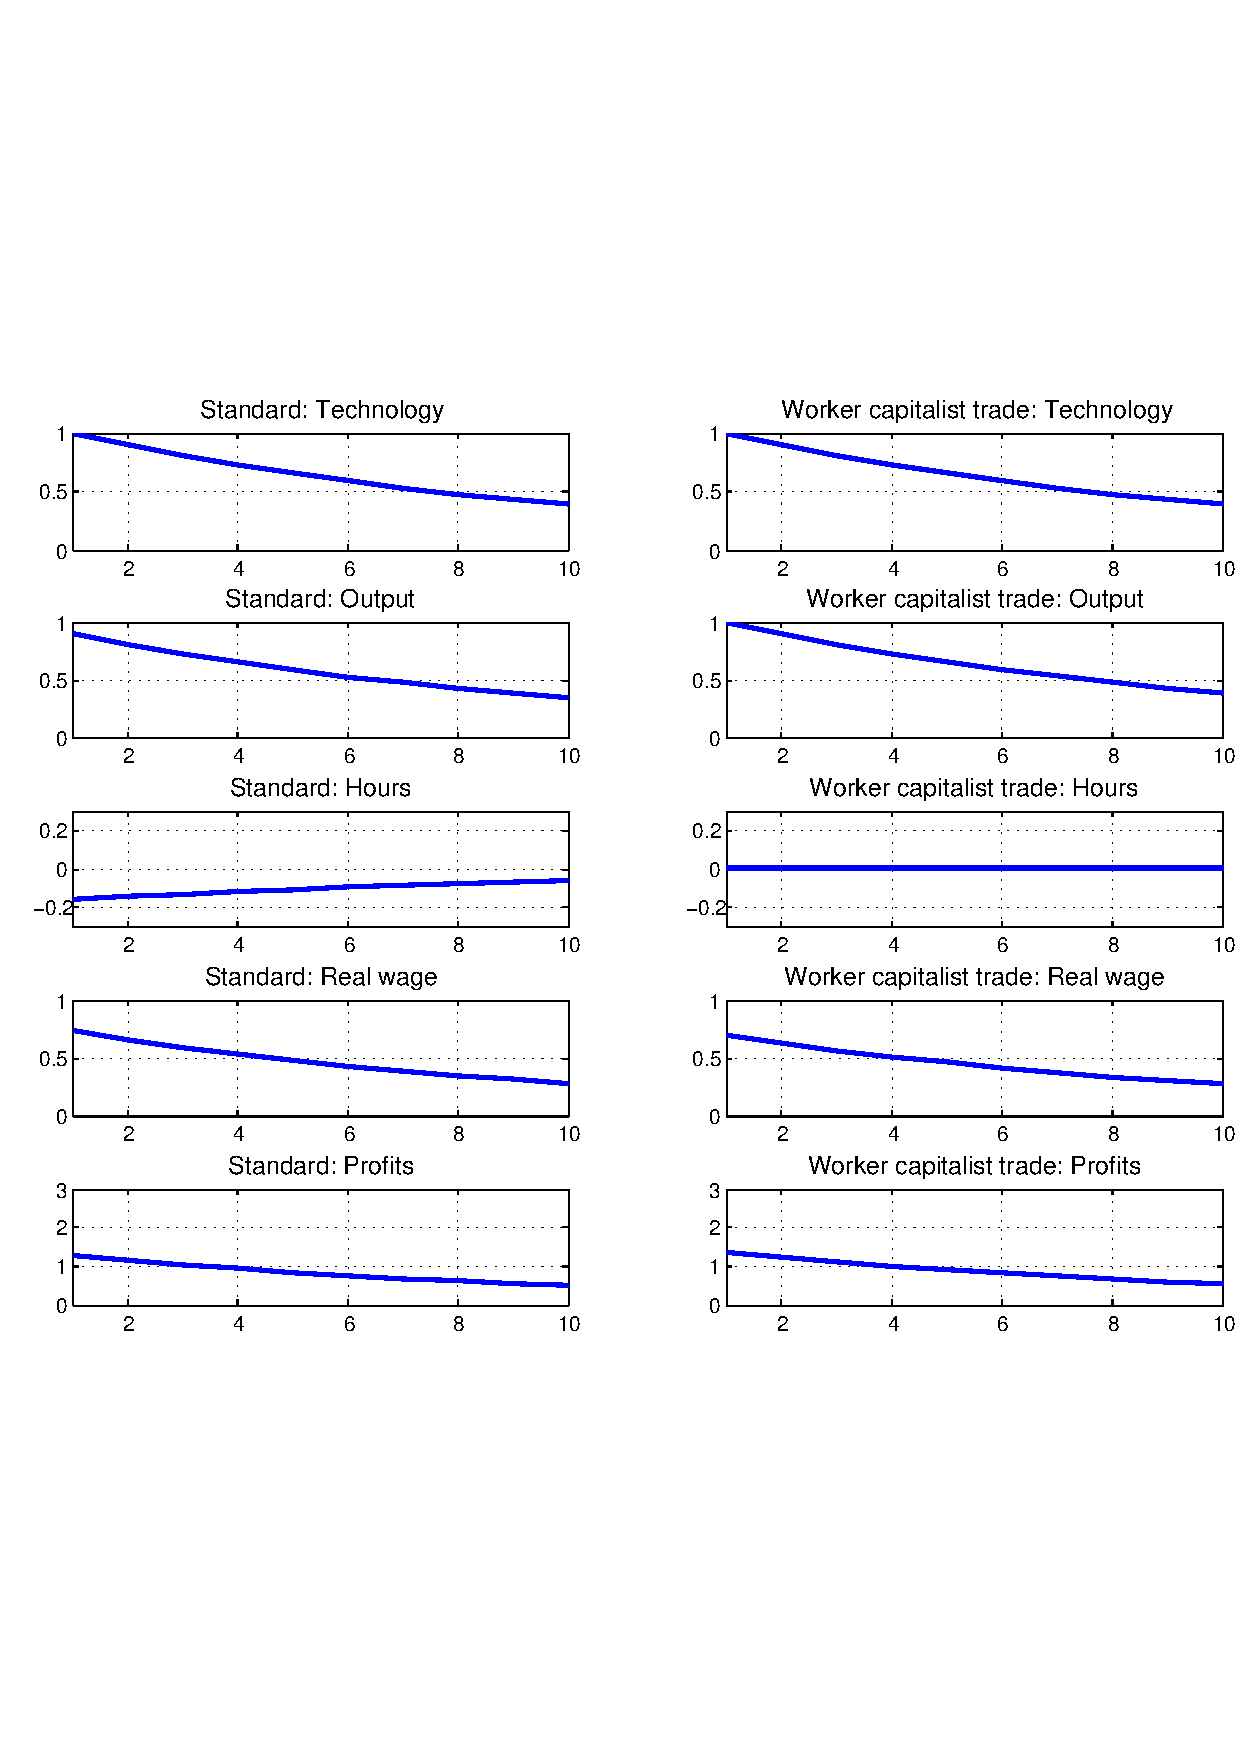
\includegraphics[trim=0.3cm 7cm 0cm 6cm, clip, width=\textwidth]{./figures/tfp_std_nt.pdf} 
\caption{Equilibrium responses to positive 1 percentage point shock in TFP. The left panel shows the standard model, the right panel the worker-capitalist model.} 
\label{fig_tfp_std_nt} 
\end{figure}


\section{Derivations and Proofs}
\lb{derivations}




\end{document}


\subsection{The 3-equation formulation of the two models}
\colorbox{red}{Discuss with co-authors!} Both models can be summarized by three linear equations.\footnote{Complete this} We derive these in the appendix, and only state them here: 
\begin{eqnarray}
\lb{wc_phillips}
\pi_t &=& \beta E_t \pi_{t+1}+\kappa_{m} \tilde{y}_t \\
\lb{wc_dis}
\tilde{y}_t &=& -\upsilon_{m} \left(i_t-E_t \pi_{t+1}-\rho\right)+E_t \tilde{y}_{t+1} \\
\lb{wc_taylor}
i_t &=& \beta + \phi_{\pi} \pi_t + \phi_{\pi} \tilde{y}_t + \nu_t 
\end{eqnarray} 
where the $m \in \{wc, std\}$ denotes a model-specific parameter.


$\kappa_{wc}=\frac{1+\varphi-(1-\sigma)(1-\alpha)}{(1-\sigma)(1-\alpha+\alpha \epsilon)}\frac{(1-\theta) (1-\beta \theta)}{\theta}$ and $ \upsilon_{wc}=\frac{(1-\sigma)(1-\alpha
)}{\sigma(1+\varphi)}$.






Former Appendix::






In this appendix, we derive the Phillip curve, the DIS curve and the equation for the natural real interest rate of the worker-capitalist model, \eqref{wc_phillips}, \eqref{wc_dis} and \eqref{wc_naturalrate}.

Of any variable $X_t$, $\bar{X}$ the steady state value, $x_t$ denotes the log, $\hat{x}_t$ the log deviation from the steady state and $\tilde{x}_t$ the log deviation from the flex price equilibrium.
% with one exception. That is that we define $g_t \equiv \log (1+\tau_t)$. 

\subsection{The Phillips curve}

In the worker-capitalist model the intermediate firms are controlled by the capitalists. The later discount consumption across time by means of the discount factor $\beta$. Thus, compared to the standard model the market discount factor, $Q_{t,t+k}$, in the firms' problem is replaced by $\beta^k$.
\begin{eqnarray}
\max_{P^*_t} &&  \sum_{k=0}^{\infty} \theta^k E_t \beta^k \left\{ P^*_t Y_{t+k|t}-\Psi_{t+k}(Y_{t+k|t})\right\} \label{eq:firm_prob_wc} \\
&& \text{s.t.}  \Psi_{t+k}(Y_{t+k|t})=\frac{W_{t+k}}{P_{t+k}}\left(\frac{N_{t+k|t}}{A_{t+k}}\right)^{\frac{1}{1-\alpha}} \nonumber \\
&&  Y_{it} = \left(\frac{P_{it}}{P_t}\right)^{-\epsilon}Y_t \nonumber
\end{eqnarray} 
The solution is characterized by
\begin{eqnarray}
\lb{int_foc_wc}
\sum_{k=0}^{\infty} \theta^k E_t \left\{ \beta^k Y_{t+k|t} (P_t^* - \mathcal{M} \psi_{t+k|t}) \right\}=0
\end{eqnarray}
where $\psi_{t+k|t}=\frac{\partial \Psi_{t+k}(Y_{t+k|t})}{\partial Y_{t+k|t}}$ and $\mathcal{M}=\frac{\epsilon}{\epsilon-1}$ is the markup over marginal cost that would have prevailed under flexible price setting $(\theta=0)$.

Now define $\Pi_{t,t+k}=\frac{P_{t+k}}{P_t}$ and $MC_{t+k|t}=\frac{\psi_{t+k|t}}{P_{t+k}}$ to get
\begin{eqnarray}
\sum_{k=0}^{\infty} \theta^k E_t \left\{\beta^{k}Y_{t+k|t}\left(\frac{P^*_t}{P_{t-1}}-\mathcal{M}MC_{t+k|t}\Pi_{t-1,t+k}\right)\right\}=0
\end{eqnarray}
Log-linearizing this equation around the steady state gives us
\begin{eqnarray}
\lb{step}
p^*_t-p_{t-1}=(1-\beta \theta) \sum_{k=0}^{\infty} (\beta \theta)^k E_t \left\{\hat{mc}_{t+k|t} + (p_{t+k}-p_{t-1}) \right\}
\end{eqnarray}
Notice that this equation is identical to the similar equation in the standard model.\footnote{\emph{E.g.} page 45 in \cite{Gali2009}}. This goes to show that letting capitalists own the firm does not changes the log-linearised optimality condition for pricing. The reason is that $Q_{t,t+k}=\beta^k$ holds in the steady state in the standard model. 

We aim to derive an expression for the individual firm's marginal cost as a function of the average marginal cost in the economy. From the labor market clearing condition \eqref{labor_clearing}, production function \eqref{tech} and demand function \eqref{demand} we get
\begin{eqnarray}
N_t &=& \int_{i=0}^{1} N_{it} di \\
&=& \int_{i=0}^{1} \left(\frac{Y_{it}}{A_t}\right)^{\frac{1}{1-\alpha}} di \\
\lb{step1}
&=& \left(\frac{Y_{t}}{A_t}\right)^{\frac{1}{1-\alpha}} \int_{i=0}^{1} \left(\frac{P_{it}}{P_t}\right)^{\frac{-\epsilon}{1-\alpha}} di
\end{eqnarray}
The integral in \eqref{step1} is measure of price dispersion which can be shown to be unity to a first order approximation. Taking logs, we get
\begin{eqnarray}
\lb{step2}
y_t=a_t+(1-\alpha)n_t
\end{eqnarray}
The economy's average marginal cost is defined by
\begin{eqnarray}
mc_t &=& (w_t-p_t)-mpn_t \\
&=& (w_t-p_t)-\frac{1}{1-\alpha}(a_t-\alpha y_t) - \log (1-\alpha)
\end{eqnarray}
An individual firms expected marginal cost in period $t+k$ if resetting price in period $t$ is
\begin{eqnarray}
mc_{t+k|t} &=& (w_{t+k}-p_{t+k})-mpn_{t+k|t} \\
 &=& (w_{t+k}-p_{t+k})-\frac{1}{1-\alpha}(a_{t+k}-\alpha y_{t+k|t}) - \log (1-\alpha)
\end{eqnarray}
Using the demand function \eqref{demand}, we can thus write
\begin{eqnarray}
\lb{step3}
mc_{t+k|t} &=& mc_{t+k}-\frac{\alpha \epsilon}{1-\alpha} (p^*_t-p_{t+k})
\end{eqnarray}
Substituting \eqref{step3} into \eqref{step}, we get
\begin{eqnarray}
p^*_t-p_{t-1}=(1-\beta \theta) \sum_{k=0}^{\infty} (\beta \theta)^k E_t \left\{ \Theta \hat{mc}_{t+k} + (p_{t+k}-p_{t-1}) \right\}
\end{eqnarray}
where $\Theta=\frac{1-\alpha}{1-\alpha+\alpha \epsilon}$ which can be rewritten as
\begin{eqnarray}
p^*_t-p_{t-1}=\beta \theta E_t \left\{p^*_{t+1}-p_t\right\}+(1-\beta \theta ) \Theta \hat{mc}_t+\pi_t 
\end{eqnarray}
Using the law of motion for inflation \eqref{prices_lom} we get that
\begin{eqnarray}
\lb{phillips_intstep}
\pi_t=\beta E_t pi_{t+1} + \lambda \hat{mc}_t
\end{eqnarray}
where $\lambda=\frac{(1-\theta) (1-\beta \theta)}{\theta } \Theta$.

We now derive an expression for $\hat{mc}_t$. The labor f.o.c. \eqref{labor_foc} implies that
\begin{eqnarray}
\lb{step4}
w_t-p_t &=& \sigma c_{wt}+\varphi n_t
\end{eqnarray}
From the workers budget constraint \eqref{worker_bc} we get that
\begin{eqnarray}
(w_t-p_t)+n_t &=&  c_{wt} \label{step5}
\end{eqnarray} 
Combining \eqref{step4} and \eqref{step5} we get that
\begin{eqnarray}
\lb{step6}
w_t-p_t =\frac{\sigma + \varphi}{1-\sigma} n_t
\end{eqnarray}
Turning to $mc_t$, \eqref{step5} and production technology \eqref{tech} implies that 
\begin{eqnarray}
mc_t &=& (w_t-p_t)-mpn_t \\
\lb{step7}
&=& \frac{1+\varphi-(1-\sigma)(1-\alpha)}{(1-\sigma)(1-\alpha)}y_t-\frac{1+\varphi}{(1-\sigma)(1-\alpha)}a_t -\log(1-\alpha)
\end{eqnarray}
Under flexible prices we know that $mc_t=-\mu \equiv \log \mathcal{M}$. Hence, we define the natural level of output $y^n_t$ from
\begin{eqnarray}
\lb{step8}
-\mu &=& \frac{1+\varphi-(1-\sigma)(1-\alpha)}{(1-\sigma)(1-\alpha)}y^n_t-\frac{1+\varphi}{(1-\sigma)(1-\alpha)}a_t -\log(1-\alpha)
\end{eqnarray}
Subtracting \eqref{step8} from \eqref{step7} we get
\begin{eqnarray}
\lb{step9}
\hat{mc}_t=\frac{1+\varphi-(1-\sigma)(1-\alpha)}{(1-\sigma)(1-\alpha)}\tilde{y}_t
\end{eqnarray}
Substituting \eqref{step9} into \eqref{phillips_intstep} we get the final Phillips curve
\begin{eqnarray}
\pi_t=\beta E_t pi_{t+1} + \kappa_{wc} \tilde{y}_t
\end{eqnarray}
where $\kappa_{wc}=\frac{1+\varphi-(1-\sigma)(1-\alpha)}{(1-\sigma)(1-\alpha+\alpha \epsilon)}\frac{(1-\theta) (1-\beta \theta)}{\theta}$


\subsection{The DIS curve}
The DIS curve in the worker-capitalist model \eqref{wc_dis} is derived from the workers' Euler equation \eqref{euler}, which in logs reads:
\begin{eqnarray}
\lb{step9}
c_{wt}=E_t c_{wt+1}-\frac{1}{\sigma}(i_t-E_t \pi_{t+1}-\rho)
\end{eqnarray}
We write this equation in deviations from the flex price equilibrium:
\begin{eqnarray}
\lb{step10}
\tilde{c}_{wt}=\tilde{c}_{wt+1}-\frac{1}{\sigma}(i_t-E_t \pi_{t+1}-r^n_t)
\end{eqnarray} 
with
\begin{eqnarray}
\lb{int_natural}
r^n_t \equiv \rho+\sigma \Delta c^n_{wt+1}
\end{eqnarray}
where $c^n_{wt}$ is the equilibrium level of consumption under flexible prices.

Next we find an expression for $\tilde{c}_{wt}$. We use \eqref{step3}, \eqref{step4} and the production technology \eqref{tech} to get
\begin{eqnarray}
\lb{step11}
c_{wt}=\frac{1+\varphi}{(1-\sigma)(1-\alpha)}(y_t-a_t)
\end{eqnarray} 
and so 
\begin{eqnarray}
\lb{step12}
\tilde{c}_{wt}=\frac{1+\varphi}{(1-\sigma)(1-\alpha)}\tilde{y}_t
\end{eqnarray}

Finally, substituting \eqref{step12} into \eqref{step10}, we get the DIS curve
\begin{eqnarray}
\tilde{y}_{t}=\tilde{y}_{t+1}-\hat{\upsilon}(i_t-E_t \pi_{t+1}-r^n_t)
\end{eqnarray}
where $\upsilon_{wc}=\frac{(1-\sigma)(1-\alpha
)}{\sigma(1+\varphi)}$.

\subsection{The natural real interest rate}
Here we derive the expression for the natural real interest rate \eqref{wc_naturalrate}. It is defined by \eqref{int_natural}. Using \eqref{step11} we get that
\begin{eqnarray}
\lb{step13}
r^n_t=\rho+\frac{\sigma (1+\varphi)}{(1-\sigma)(1-\alpha)} \left(\Delta y^n_{t+1}-\Delta a_{t+1} \right)
\end{eqnarray}
From \eqref{step8} we get an expression for the natural output gap
\begin{eqnarray}
y^n_t=-\frac{(\mu-\log(1-\alpha))(1-\sigma)(1-\alpha)}{1+\varphi-(1-\sigma)(1-\alpha)} + \frac{1+\varphi}{1+\varphi-(1-\sigma)(1-\alpha)}a_t
\end{eqnarray}
and so
\begin{eqnarray}
\lb{step14}
\Delta y^n_{t+1}= \frac{1+\varphi}{1+\varphi-(1-\sigma)(1-\alpha)}\Delta a_{t+1}
\end{eqnarray}
Substituting \eqref{step14} into \eqref{step13} we get the expression for the natural level of the real interest rate:
\begin{eqnarray}
r^n_t=\rho+\xi^a_{wc} \Delta a_{t+1} 
\end{eqnarray}
where $\xi^a_{wc}=\frac{\sigma (1+\varphi)}{1+\varphi-(1-\sigma)(1-\alpha)}$.